\documentclass[slovene,11pt,a4paper]{article}
\usepackage[margin=1.8cm,bottom=3cm,foot=1.5cm]{geometry}
\usepackage{amsmath}
\usepackage{booktabs}
\usepackage{float}
\usepackage{graphicx}
\usepackage{gensymb}
\usepackage{geometry}
\usepackage{changepage}
\usepackage{subcaption}
\usepackage{multirow}
\usepackage{blindtext}
\usepackage{hyperref}
\usepackage[slovene]{babel}
\pagenumbering{gobble}
\renewcommand{\contentsname}{\centering Contents}

\begin{document}

\title{1. naloga - Model vožnje skozi semafor: variacijska metoda}
\author{Tadej Lozej 28201055}
\maketitle
\begin{center}
Modelska analiza 1 \\
\bigskip
Predavatelj: prof. dr. Simon Širca \\
Asistent: doc. dr. Miha Mihovilovič
\end{center}

\newpage

\tableofcontents

\newpage

\section{Uvod}

\pagenumbering{arabic}

V nalogi smo modelirali vožnjo avta skozi semafor. Z avtom želimo priti do semaforja ravno, ko se prižge zelena luč. Vemo, da se v nekem trenutku nahajamo na razdalji $L$ pred semaforjem in , da bo rdeča luč gorela še $T$ časa. Proti semaforju se ob tem trenutku vozimo s hitrostjo $v_0$. Vožnjo optimiziramo na več načinov in prav tako obravnavamo več možnih scenarijev na cesti.

\section{Začetni problem}

Formuliramo problem začetne obravnave. Za začetek navedimo prvi pogoj, ki pravi, da do semaforja pridemo ravno, ko se rdeča luč ugasne oz. ravno, ko se prižge zelena. Ta pogoj podamo z integralom hitrosti po času

\begin{equation}
\int\limits_{0}^{T} v(t) dt = L.
\end{equation}
Ker pa želimo do semaforja priti z varčno in udobno vožnjo moramo definirati tudi pogoj udobnosti vožnje. Tega se da formulirati na več načinov. Eden izmed možnih načinov je z minimizacijo integrala kvadrata pospeška po poti avta do semaforja

\begin{equation}
\int\limits_{0}^{T} \dot{v}(t)^2 dt = min.
\end{equation}
Vidimo, da je to variacijski problem. Pristopimo z Lagrangevo funkcijo

\begin{equation}
L(\dot{v}, v) = \dot{v}^2 - \lambda v,
\end{equation}
kjer je $\lambda$ Lagrangev multiplikator. Euler-Lagrangeve enačbe nam dajo splošno rešitev problema

\begin{equation}
v = \frac{\lambda}{4} t^2 + At + B.
\end{equation}

Koeficienta $A$ in $B$ določimo iz robnih pogojev, multiplikator $\lambda$ pa iz prvega pogoja oz enačbe (1). Pri robnih pogojih $v(0) = v_0$ in $\dot{v}(T) = 0$ dobimo rešitev

\begin{equation}
v(t) = v_0 + \frac{3(L-v_0 T)}{2T^3} (2Tt-t^2).
\end{equation}
To lahko prepišemo v brezdimenzijsko obliko z novo definiranimi  brezdimenzijskimi spremenljivkami $\tau = \frac{t}{T}$, $\chi = \frac{x}{L}$ in $\nu = \frac{v}{V}$, kjer je $V = \frac{L}{T}$. Enačba (5) z brezdimenzijskimi spremenljivkami napišemo

\begin{equation}
\nu(\tau) = \nu_0 + \frac{3}{2}(1-\nu_0)(2\tau-\tau^2),
\end{equation}
kjer je $\nu_0 = \frac{v_0}{V}$. Seveda je ničla polinoma odvisna od njegovih koeficientov, zato bo model, odvisno od izbire $\nu_0$, morda imel ničlo med 0 in 1, kar pomeni, da bo avto na poti do semaforja spremenil smer hitrosti. Se pravi bo semafor prevozil in nato vozil do njega vzvratno. To seveda ni v redu in pri takšnih vrednostih $\nu_0$ naš model odpove, saj ne upošteva cestno prometnih predpisov. Slika 1 prikazuje enačbo (6) pri nekaj različnih vrednostih $\nu_0$. Na njej lepo vidimo, da se omenjen priblem zgodi pri vrednosti $\nu_0 > 3$.

Če integriramo enačbo (5), dobimo pot v odvisnosti od časa $x(t)$, ki jo prav tako lahko prepišemo v brezdimenzijsko obliko

\begin{equation}
\chi(\tau) = \nu_0 \tau + \frac{1-\nu_0}{2}(3\tau^2 - \tau^3).
\end{equation}
Brezdimenzijska pot v odvisnosti od brezdimenzijskega časa je prikazana na sliki 2.
\newpage

\begin{figure}[h!]
\centering
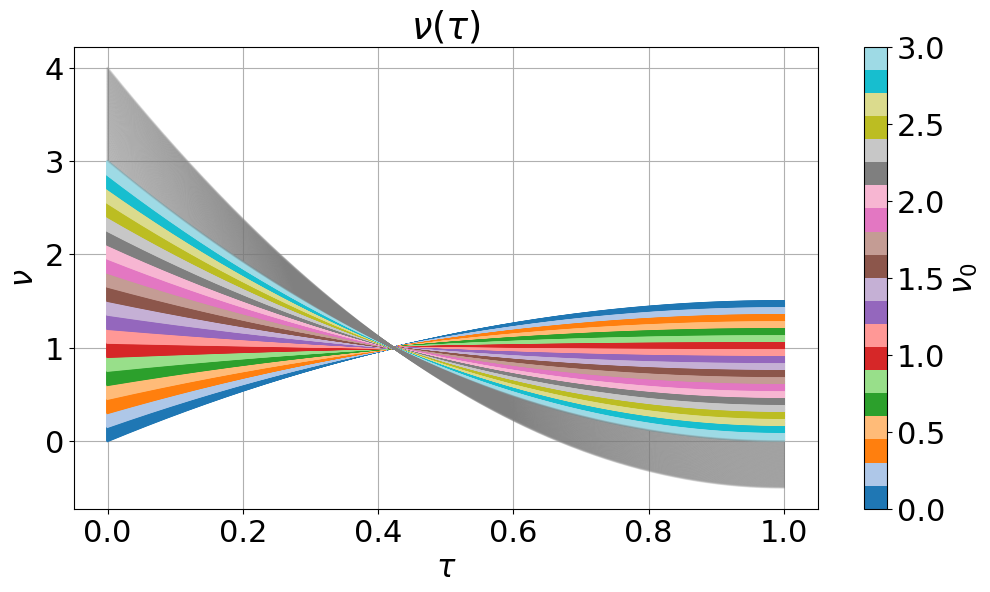
\includegraphics[width=\linewidth]{ZacetniProblem1.png}
\caption{Enačba (6) pri različnih vrednostih začetne brezdimenzijske hitrosti $\nu_0$. Pri vrednosti $\nu_0 > 3$ vsebuje zaloga vrednosti funkcije tudi negativne brezdimenzijske hitrosti.}
\end{figure}

\begin{figure}[h!]
\centering
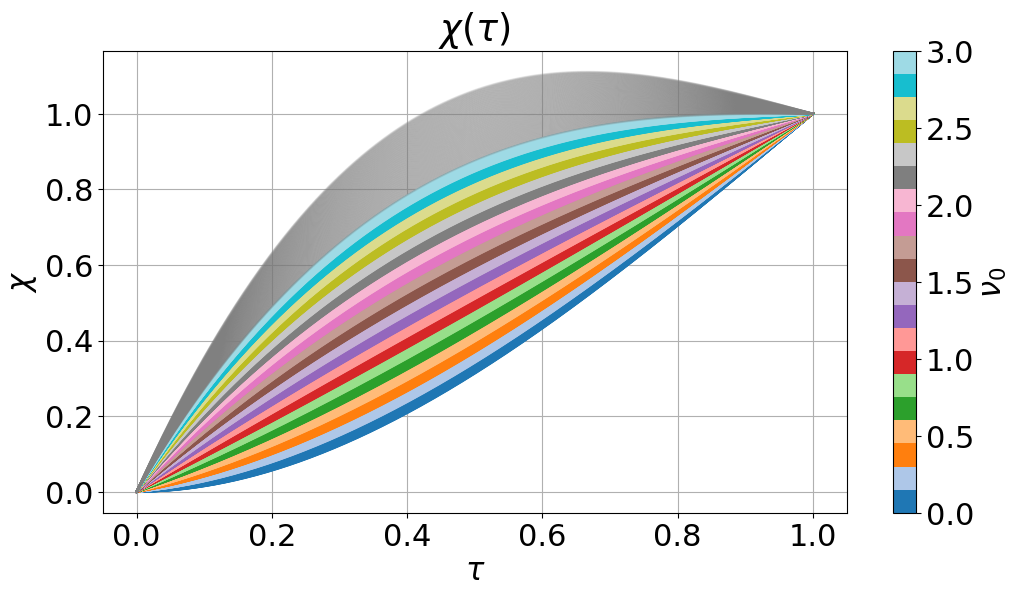
\includegraphics[width=\linewidth]{ZacetniProblem2.png}
\caption{Enačba (7) pri različnih vrednostih začetne brezdimenzijske hitrosti $\nu_0$. Pri vrednosti $\nu_0 > 3$ vsebuje zaloga vrednosti funkcije večje od 1.}
\end{figure}

Zanimivo je, da pri se pri grafu brezdimenzijske hitrosti v odvisnosti od brezdimenzijskega časa (slika 1) vse krivulje sekajo pri vrednosti $\tau = 1 - \frac{1}{3}$ neodvisno od parametra $\nu_0$. Na sliki 3 je prikazana tudi brezdimenzijska hitrost v odvisnosti od brezdimenzijske koordinate pri par različnih vrednostih $\nu_0$. Graf sem dobil tako, da sem si zapomnil točke ($\chi$, $\nu$) pri več različnih časih $\tau$ in nato narisal graf $\nu(\chi)$.

\begin{figure}[h!]
\centering
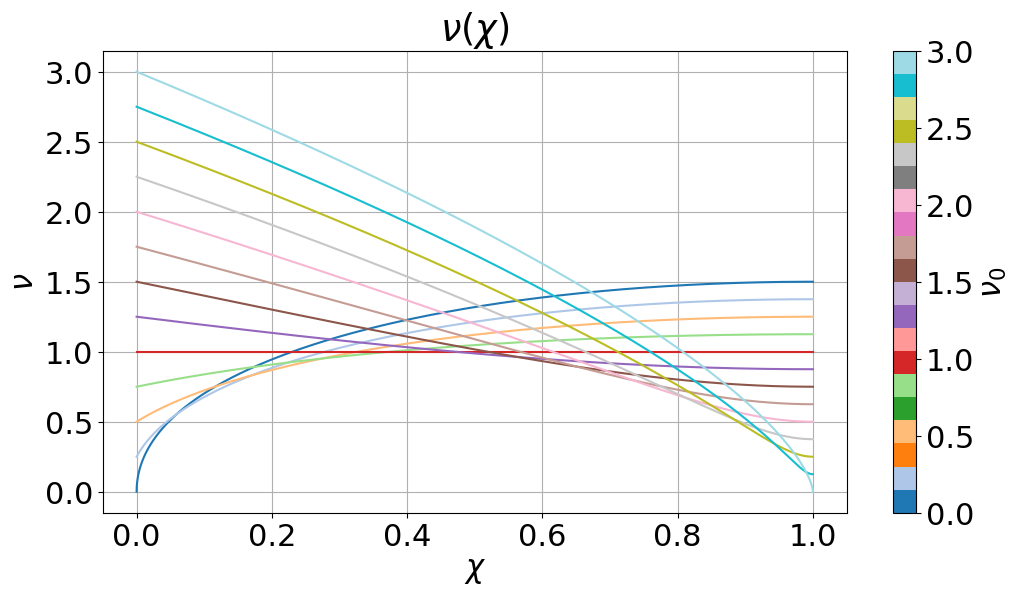
\includegraphics[width=\linewidth]{ZacetniProblem3.png}
\caption{Brezdimenzijska hitrost $\nu$ v odvisnosti od brezdimenzijske koordinate $\chi$ pri nekaj različnih vrednostih $\nu_0$.}
\end{figure}

\section{Radar pri semaforju}

Obravnavajmo isti primer a z enim drugačnim robnim pogojem. Recimo, da je pri semaforju radar, mimo katerega želimo peljati s hitrostjo $v_max$. Tako se drugi robna pogoja glasita $v(0) = v_0$ in $v(T) = v_max$. Poleg teh dveh pogojev mora prav tako še vedno veljati enačba (1). Splošna rešitev je še vedno parabola. Iz enačbe (4) z novimi robnimi pogoji določimo nove koeficiente $A$, $B$ in $\lambda$ in dobimo enačbo za hitrost v odvisnosti od časa

\begin{equation}
v(t) = \frac{3(2L - v_0T - v_{max}T)}{T^3} (Tt-t^2) + \frac{v_{max} - v_0}{T} t + v_0.
\end{equation}
To lahko kot v prejšnjem primeru prepišemo v brezdimenzijsko obliko

\begin{equation}
\nu(\tau) = 3(2 - \nu_0 - \nu_{max})(\tau - \tau^2) + (\nu_{max} - \nu_0)\tau + \nu_0,
\end{equation}
kjer je $\nu_{max} = \frac{v_{max}}{V}$. Izberemo si vrednost parametra $\nu_{max} = 1$ in izrišemo kvadratne funkcije enačbe (9) za različne vrednosti parametra $\nu_0$ (slika 4). Vidimo, da rešitve s parametrom $\nu_0 > 4$ spet niso aplikativne, saj ne upoštevajo cestno prometnih predpisov, ker se bi po cesti vozili vzvratno.

\begin{figure}[h!]
\centering
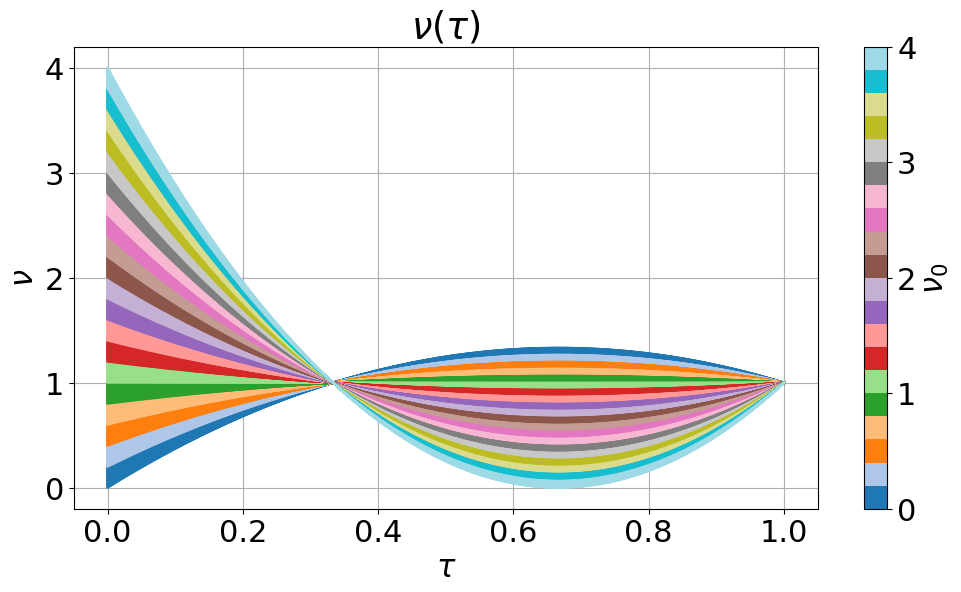
\includegraphics[width=\linewidth]{Radar1.png}
\caption{Enačba (9) pri različnih vrednostih začetne brezdimenzijske hitrosti $\nu_0$. Rešitve z parametrom $\nu_0 > 4$ ne upoštevajo cestno prometnih predpisov in jih zato ne upoštevamo.}
\end{figure}

Če enačbo (8) integriramo po času kot prej dobimo koordinato x avta v odvisnosti od časa. Enačbo nato prepišemo še v brezdimenzijsko obliko

\begin{equation}
\chi(\tau) = (2-\nu_0-\nu_{max})\left(\frac{3}{2}\tau^2 - \tau^3 \right) + \frac{\nu_{max} - \nu_0}{2} \tau^2 + \nu_0 \tau.
\end{equation}
Brezdimenzijska koordinata v odvisnosti od brezdimenzijskega časa $\chi(\tau)$ je prikazana na sliki 5. 

\newpage

\begin{figure}[h!]
\centering
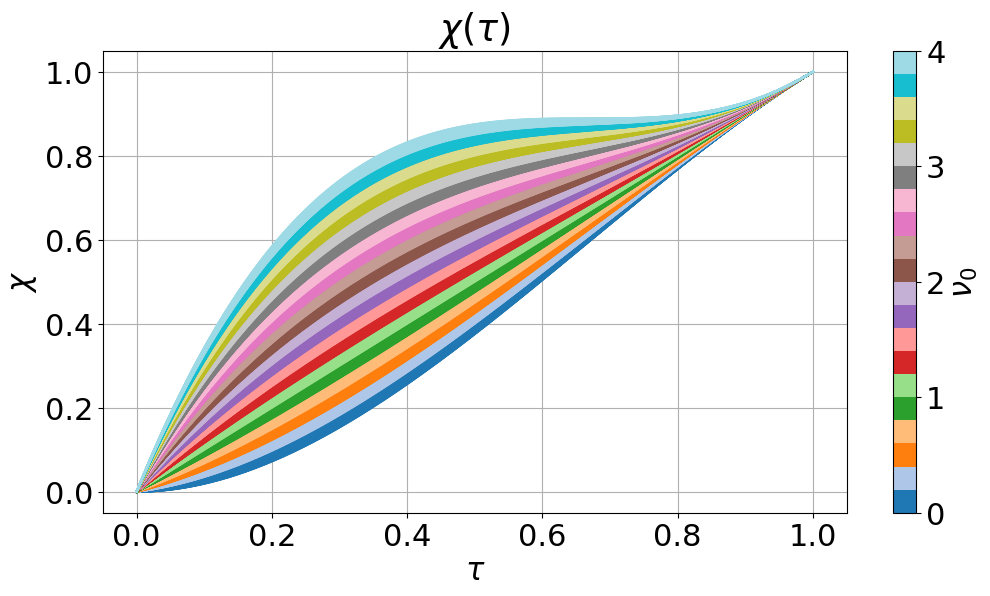
\includegraphics[width=\linewidth]{Radar2.png}
\caption{Enačba (10) pri različnih vrednostih začetne brezdimenzijske hitrosti $\nu_0$.}
\end{figure}

Podobno kot v prejšnjem poglavju se tudi v tem primeru lahko znajdemo in narišemo tudi graf brezdimenzijske hitrosti $\nu$ v odvisnosti od brezdimenzijske koordinate $\chi$ pri par različnih začetnih hitrostih $\nu_0$.

\begin{figure}[h!]
\centering
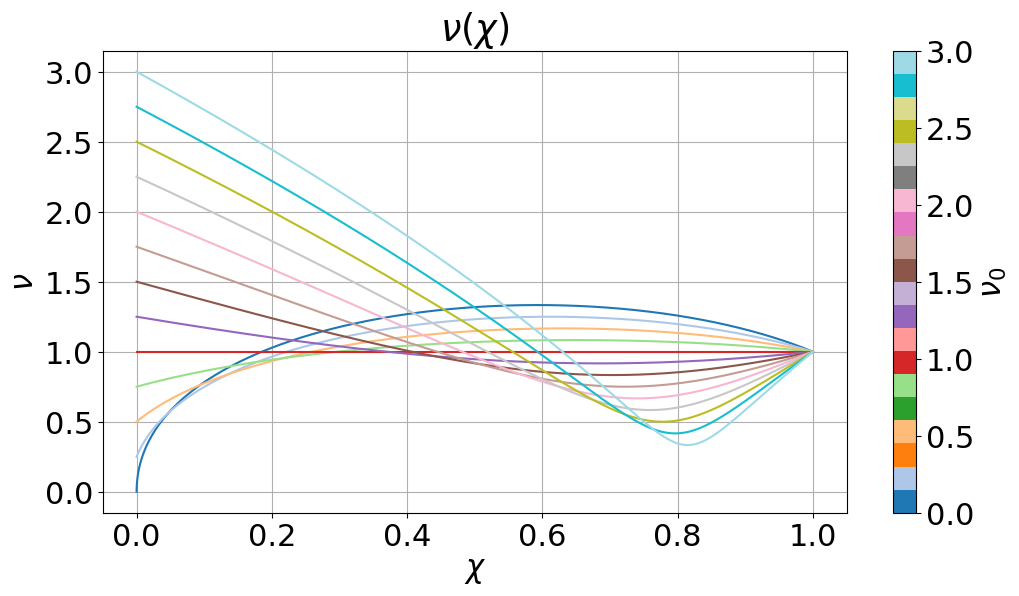
\includegraphics[width=\linewidth]{Radar3.png}
\caption{Brezdimenzijska hitrost v odvisnosti od brezdimenzijske koordinate $\chi$, pri par različnih vrednostih $\nu_0$.}
\end{figure}

\section{Sode potence v funkcionalu}

Do sedaj smo pogoj udobnosti definirali kot minimum kvadrata pospeška po poti avta, enačba (2). Poglejmo si še več načinov s katerimi lahko formuliramo udobno vožnjo. Kaj če minimiziramo integral višjih sodih potenc pospeška

\begin{equation}
\int\limits_{0}^{T} \dot{v}(t)^{2p} dt = min,
\end{equation}
kjer je $p$ naravno število. Na ta način še bolj kaznujemo večje pospeške in slutimo, da bodo spremembe hitrosti počasnejše. Imamo nov funkcional

\begin{equation}
L(\dot{v}, v) = \dot{v}^{2p} - \lambda v,
\end{equation}
ki da nove Euler-Lagrangeove enačbe in tako novo splošno rešitev za hitrost v odvisnosti od časa

\begin{equation}
v(t) = - \frac{2p-1}{\lambda} \left(C-\frac{\lambda t}{2p}\right)^{\frac{2p}{2p-1}} + D.
\end{equation}
Tukaj sta $C$ in $D$ konstanti določeni iz robnih pogojev problema in $\lambda$ Lagrangev multiplikator določen z enačbo (1).

Izberimo si robne pogoje kot v poglavju 1 $v(0) = v_0$ in $\dot{v}(T) = 0$. Dobimo rešitve za koeficiente

\[
C = \frac{\lambda T}{2p}, \quad
D = v_0 + \frac{2p-1}{\lambda} C^{\frac{2p}{2p-1}} \quad \text{in} \quad
\lambda = \left( \frac{2p}{T} \right)^{2p} \left[\frac{L/T - v_0}{(2p-1) (1-(2p-1)/(4p-1))}\right]^{2p-1}.
\]

Če v izraz za $\lambda$ vstavimo $p=1$ dobimo enako vrednost $\lambda$ kot v prbem poglavju naloge, kar vzamem za dovolj dober znak, da je izraz pravi. S temi koeficienti nadaljujemo in tako dobimo izraz za brezdimenzijsko hitrost

\begin{equation}
\nu(\tau) = \nu_0 + \frac{4p-1}{2p}(1-\nu_0)\left[1-(1-\tau)^{\frac{2p}{2p-1}}\right].
\end{equation}
Preden enačbo (14) narišemo na graf razislimo še o limiti $p\rightarrow \infty$. Večji kot je $p$ bolj kaznujemo velike pospeške in pojemke. Zato sklepamo, da se bo ta hitro ustalil na neki konstantni vrednosti in bomo v limiti premo enakomerno pospešenega gibanja. V limiti upoštevamo pravilo limite racionalne funkcije. Če sta polinoma v števcu in imenovalcu iste stopnje je limita razmerje vodilnih členov. Tako velja

\begin{equation}
\lim\limits_{p\rightarrow \infty} \nu(\tau) = \nu_0 + 2(1-\nu_0)\tau.
\end{equation}
Na sliki 5 je graf enačbe (14) z nekaj različnimi vrednostmi $p$ in parametrom $\nu_0 = 0$.

\begin{figure}[h!]
\centering
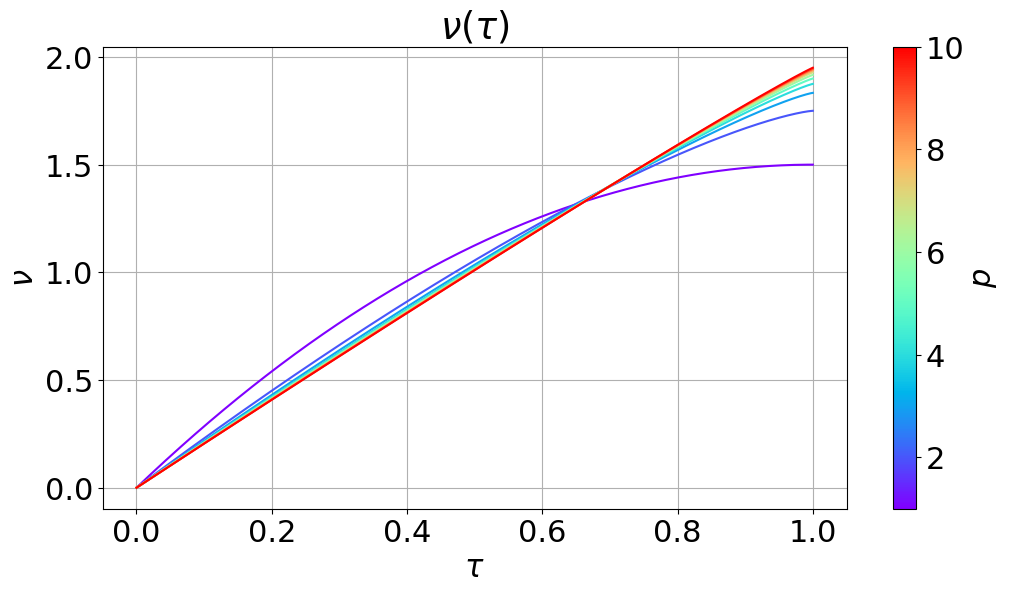
\includegraphics[width=\linewidth]{SodePotence1.png}
\caption{Enačba (14) pri različnih vrednostih parametra $p$. V limiti $\lim\limits_{p\rightarrow \infty}$ se graf približuje premici iz enačbe (15).}
\end{figure}

\section{Kvadrat hitrosti v funkcionalu}

Pogoj udobnosti smo do sedaj definirali le s pomočjo minimizacije različnih potenc pospeška. Kaj pa, če nam udobna počasnejša vožnja? V integral, ki ga minimiziramo, dodajmo še kvadratni člen hitrosti

\begin{equation}
\int\limits_{0}^{T} \left( \dot{v}(t)^2 + C v^2 \right) dt = min,
\end{equation}
kjer je $C$ prost parameter. Z večjim $C$ bolj zahtevamo počasnejšo vožnjo. Funkcional je v tem primeru

\begin{equation}
L(\dot{v}, v) = \dot{v}^2 + v^2 = -\frac{\lambda}{2}
\end{equation}
in diferencialna enačba, ki jo dajo Euler-Lagrangeve enačbe je 

\begin{equation}
\ddot{v} - Cv = - \frac{\lambda}{2}.
\end{equation}
To je nehomogena linearna diferencialna enačba. Homogeno rešitev poiščemo z nastavkom $v^{HOM} = Ae^{\alpha t} \Rightarrow v^{HOM} = A_1 e^{\sqrt{C}t} + A_2 e^{-\sqrt{C}t}$, partikularno pa uganemo $v^{PART} = \frac{\lambda}{2C}$. Konstanti $A_1$ in $A_2$ določimo iz robnih pogojev enakih kot v poglavju 1 $v(0) = v_0$ in $\dot{v}(T) = 0$, multiplikator $\lambda$ pa iz enačbe (1). Dobimo

\[
A_1 = \frac{v_0 - \lambda/(2C)}{1+e^{2\sqrt{C}T}}, \quad
A_2 = \frac{v_0 - \lambda/(2C)}{1+e^{-2\sqrt{C}T}}, \quad \text{in} \quad
\lambda = 2C \frac{L-v_0/\sqrt{C}\tanh(\sqrt{C}T)}{T-1/\sqrt{C}\tanh(\sqrt{C}T)}.
\]

Z znanimi koeficienti lahko zapišemo hitrost $v(t)$ in v naslednjem koraku brezdimenzijsko hitrost $\nu(\tau)$

\begin{equation}
\nu(\tau) = \frac{1-\nu_0/\tau_C \tanh(\tau_C)}{1-1/\tau_C \tanh(\tau_C)} \left(
1-\frac{\cosh(\tau_C(\tau-1))}{\cosh(\tau_C)} \right) + 
\nu_0 \frac{\cosh(\tau_C(\tau-1))}{\cosh(\tau_C)},
\end{equation}
kjer je $\tau_C = \sqrt{C}T$. V primeru, kjer bo $\tau_C$ majhen pričakujemo podobno rešitev kot v prvem delu naloge. Ko bo $\tau_C$ velik pa pričakujemo, da se bo hitrost hitro ustalila na neki čim manjši možni vrednosti. Poglejmo si graf enačbe (19) za ta dva primera pri različnih vrednostih $\nu_0$.

\begin{figure}[h!]
\centering
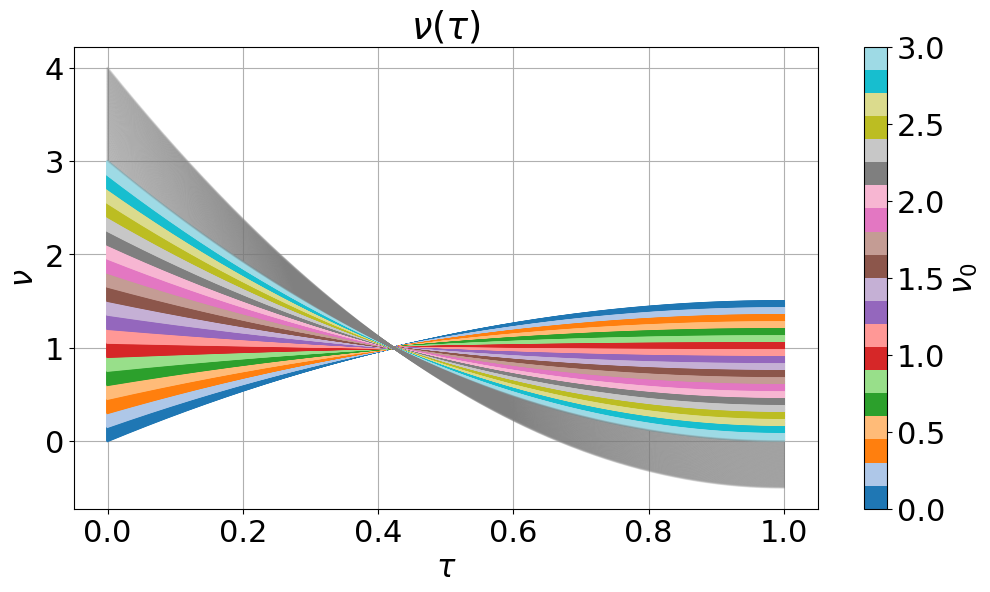
\includegraphics[width=\linewidth]{HitrostFunkcional1.png}
\caption{Enačba (19) pri različnih vrednostih parametra $\nu_0$, pri vrednosti $\tau_C = 0,001$.}
\end{figure}
Vidimo, da je slika 6 zelo podobna sliki 1, kot smo tudi pričakovali za majhen $\tau_C$. Poglejmo si še graf enačbe (19) za vrednost $\tau_C = 10$. Tukaj se hitrost hipoma ustali pri najnižji možni vrednosti, ki jo omeji enačba (1).

\newpage

\begin{figure}[h!]
\centering
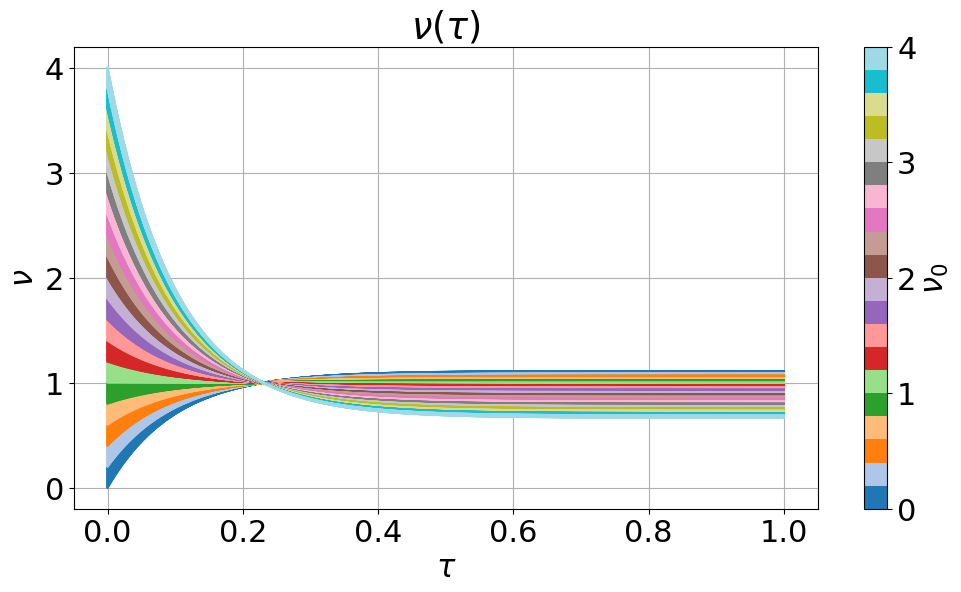
\includegraphics[width=\linewidth]{HitrostFunkcional2.png}
\caption{Enačba (19) pri različnih vrednostih parametra $\nu_0$, pri vrednosti $\tau_C = 10$.}
\end{figure}

\section{Zaporedni semaforji}

Kakšna bi pa bila optimalna vožnja skozi $N$ zaporednih semaforjev? Recimo, da so vsi semaforji na enaki medsebojni razdalji $L$ in med dvema semaforjema vozimo $T$ časa. Lahko bi mininmizirali kvadrat pospeška na vsakem odseku ceste posebej ampak poskušajmo raje minimizirati kvadrat pospeška globalno. Minimizirati želimo funkcional

\begin{equation}
L = \dot{v_1}^2 + \lambda_1 v_1 + \dot{v_2}^2 + \lambda_2 v_2 + \dot{v_3}^2 + \lambda_3 v_3 ...,
\end{equation}
kjer so $v_n$ hitrosti od $n-1$ do $n$ tega semaforja. Hitrosti $v_n$ obravnavamo kot ločene koordinate in posledično po Euler-Lagrangevih enačbah

\begin{equation}
\frac{d}{dt} \left(\frac{\partial L}{\partial \dot{v_n}} \right) - \frac{\partial L}{\partial v_n} = 0
\end{equation}
dobimo sistem enačb, katerega rešitve so parabole

\begin{equation}
v_n = - \frac{\lambda_n}{4}t^2 + A_n t + B_n.
\end{equation}

Zagotoviti želimo gladko vožnjo oz. zveznost pospeška na mejah. V vsakem odseku imamo 3 proste parametre, 2 robna pogoja (zveznost in odvedljivost) in pogoj določen z enačbo (1). Problem bi moral biti rešljiv. Robna pogoja, ki si ju lahko izberemo, sta pogoj pri začetku prvega odseka in pogoj pri koncu zadnjega. Robni pogoji izgledajo sledeče

\[
v_1(0) = v_0, \quad v_2(T) = v_1(T) \, ... \quad v_{n}((n-1)T) = v_{n-1}((n-1)T) \, ... \quad v_{N}((N-1)T) = v_{N-1}((N-1)T)
\]

\[
\dot{v}_1(T) = \dot{v}_2(T), \quad \dot{v}_2(2T) = \dot{v}_3(2T) \, ... \quad \dot{v}_{n-1}((n-1)T) = \dot{v}_{n}((n-1)T) \, ... \quad \dot{v}_{N}(NT) = 0.
\]

\newpage

Za lažjo obravnavo problem prepišemo v brezdimenzionalni. Splošna rešitev je 

\begin{equation}
nu_n = \alpha_n \tau^2 + \beta_n \tau + \gamma.
\end{equation}
Robni pogoji pa se glasijo

\[
\nu_1(0) = \nu_0, \quad \nu_2(1) = \nu_1(1) \, ... \quad \nu_{n}((n-1)) = \nu_{n-1}((n-1)) \, ... \quad \nu_{N}((N-1)) = \nu_{N-1}((N-1))
\]

\[
\dot{\nu}_1(1) = \dot{\nu}_2(1), \quad \dot{\nu}_2(2) = \dot{\nu}_3(2) \, ... \quad \dot{\nu}_{n-1}((n-1)) = \dot{\nu}_{n}((n-1)) \, ... \quad \dot{\nu}_{N}(N) = 0.
\]
in seveda na vsakem odseku moramo še vsak $v_n$ brezdimenzijsko upoštevati enačbo (1)

\begin{equation}
\int\limits^{n}_{n-1} \nu_n(\tau) d\tau = 1.
\end{equation}

Tako imamo za vsak interval tri neznanke in tri enačbe. Spodaj na sliki 

\begin{figure}[h!]
\centering
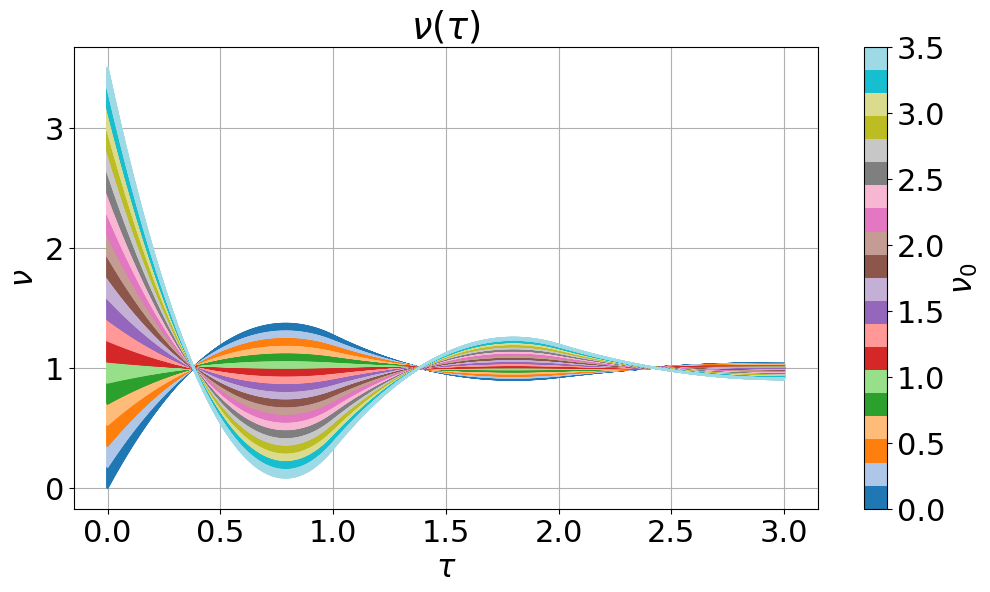
\includegraphics[width=\linewidth]{HitrostZaporedniSemaforji1.png}
\caption{Zlapljena rešitev brezdimenzijske hitrosti $\nu$ skozi tri semaforje v odvisnosti od brezdimenzijskega časa $\tau$.}
\end{figure}
Vidimo, da je optimalna vožnja takšna, da avto čim prej doseže konstantno hitrost s katero bi nato vozil premo enakomerno skozi semaforje.

\section{Zaključek}

Uspašno smo rešili in predstavili rešitve podanih problemov. Videli smo kako se različni pogoji udobnosti poznajo na vožnji avta. Prav tako smo dobili občutek za kakovost modela oz. za to kdaj model odpove. Definitivno bi model lahko še dalje nadgrajevali.


\end{document}